\scanpage{139}
U N I V E R S I T E

DES SCIENCES ET TECHNIQUES

DU LANGUEDOC

\texttt{------------}

MONTPELLIER, le 4 Juillet 1979

Service de la Scolarité

MR / GJ

Diffusion : Liste A

N° : 3929

\uline{AVIS DE SOUTENANCE D'UNE THESE DE DOCTEUR INGENIEUR}

\uline{SCIENCES ALIMENTAIRES Option GENIE ET TECHNOLOGIE ALIMENTAIRES - FERMENTATION}

\uline{Nom et prénom du candidat} :

ARJONA José Luis

\uline{Titre de la thèse} :

``Contribution à l'étude de la torréfaction en couche fluidisée''.

\uline{Date, heure et lieu de soutenance prévus} :

\uline{11 JUILLET} 1979 à 10 Heures 30 mn

Salle de cours n° 10

U. S. T. L.

\uline{Nom du Directeur de thèse} :

Monsieur H. GIBERT

\uline{Désignation du laboratoire où la thèse est préparée} :

Génie Alimentaire.

\uline{Résumé de la thèse} :

Ce travail est centré sur l'étude d'un nouveau procédé de torréfaction mettant en oeuvre une couche fluidisée. Différentes techniques ont été essayées :

- Torréfaction par fluidisation directe des grains de café dans un courant d'air chaud,

- Torréfaction par flottation - immersion au sein d'une couche fluidisée de produits inertes portée à température adéquate.

La fluidisation s'avère un excellent moyen d'étude des mécanismes de torréfaction et de détermination des conditions opératoires optimales (température).

L'intérêt du procédé est souligné sur le plan de la consommation énergétique (très faibles durées de torréfaction), comme sur celui de la qualité des produits (uniformité de traitement de la charge).

\uline{Durée approximative des recherches ayant abouti à la thèse} : 3 ans 1/2.

\uline{Composition du jury proposé} :

MM.

GIBERT

CHARREAU

COUDERC

CROUZET

DOTHEE

VINCENT

Le Secrétaire Général,

\figure{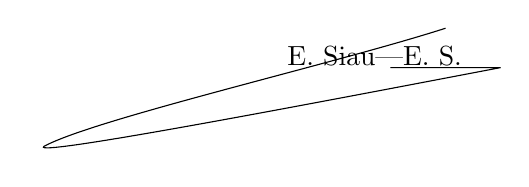
\begin{tikzpicture}[x=1cm,y=1cm]
\draw (5.1,1.5) .. controls (3.7,1.05) and (.65,.35) .. (0,0) .. controls (-.2,-.15) and (3.7,.6) .. (5.8,1.0) -- (4.4,1.0);
\node at (4.2,1.15) {\unsure{E. Siau|E. S.}};
\end{tikzpicture}}

\uline{E. S I A U}

\margin{139}
